\documentclass[11pt,table]{article}
% DEFINE COMMANDS

\usepackage{NotesTeX}

\usepackage[font=small,labelfont=bf]{caption}
\usepackage{enumerate}
\usepackage{amsmath,amssymb,amscd,amsfonts}
\usepackage{xcolor}
\usepackage{color}
\usepackage{mathrsfs}

\usepackage{tikz}
\usepackage{tikz-cd}
\tikzcdset{every label/.append style = {font = \small}}
\tikzcdset{row sep/normal=3.5em}
\tikzcdset{column sep/normal=3.5em}

\usetikzlibrary{matrix}
\usetikzlibrary{decorations.markings,calc,shapes}
\usetikzlibrary{positioning}
\usepackage{graphicx}
\usepackage{empheq}
\usepackage{physics}
\usepackage{siunitx}
\usepackage{tensor}

\usepackage{multicol}

\usepackage{youngtab}
\usepackage{cancel}
\usepackage{caption}
\usepackage{graphicx}
\usepackage{subcaption}
\usepackage{hyperref}


% added by Jingtian Shi
\usepackage{indentfirst}
\usepackage{cases}
\usepackage{bbm}

\usepackage{esvect}
\usepackage{accents}
\newcommand{\ut}[1]{\underaccent{\tilde}{#1}}
%\renewcommand{\vec}[1]{\ut{#1}}
% % % % % % % % % % % % % % % % % % % % % % %

\title{{\Huge General Relativity}\\{\Large{Class 34 --- April 17, 2020}}} %replace with class number
\author{Rabia Husain}

\emailAdd{r.husain@utexas.edu} %replace with your email
\begin{document}
\maketitle
\flushbottom
\newpage
\pagestyle{fancynotes}

\part{Stationary Black Holes}

We now want to apply our hypersurface tools from previous lectures to black hole spacetimes in order to understand more about their properties. Our goal is to understand how to detect an event horizon of a black hole. This is a global property so it is not always obvious how to do so, but in the stationary case we can do this.

Consider the Schwarzschild case, where we know the event horizon occurs at some constant $r = r_{H}$, where $r$ is a normal radial coordinate. At the event horizon, the constant $r$ hypersurface becomes null.

\begin{figure}[h]
\centering

\tikzset{every picture/.style={line width=0.75pt}} %set default line width to 0.75pt        

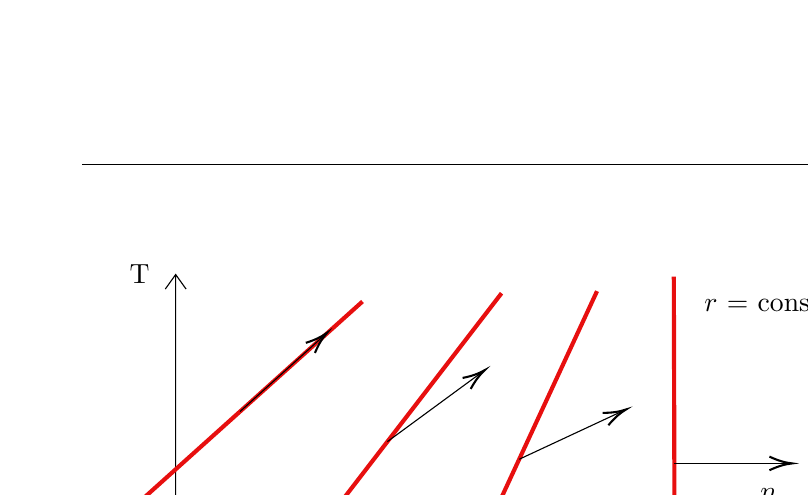
\begin{tikzpicture}[x=0.75pt,y=0.75pt,yscale=-1,xscale=1]
%uncomment if require: \path (0,242); %set diagram left start at 0, and has height of 242

%Shape: Axis 2D [id:dp0681679685979113] 
\draw  (89,197) -- (409.5,197)(120.5,16) -- (120.5,221) (402.5,192) -- (409.5,197) -- (402.5,202) (115.5,23) -- (120.5,16) -- (125.5,23)  ;
%Straight Lines [id:da23859611191862928] 
\draw [color={rgb, 255:red, 231; green, 15; blue, 15 }  ,draw opacity=1 ][line width=1.5]    (360.5,17) -- (361,197) ;
%Straight Lines [id:da7533548797688308] 
\draw    (360.75,107) -- (415.5,107) ;
\draw [shift={(417.5,107)}, rotate = 180] [color={rgb, 255:red, 0; green, 0; blue, 0 }  ][line width=0.75]    (10.93,-3.29) .. controls (6.95,-1.4) and (3.31,-0.3) .. (0,0) .. controls (3.31,0.3) and (6.95,1.4) .. (10.93,3.29)   ;
%Straight Lines [id:da9093944903331157] 
\draw [color={rgb, 255:red, 231; green, 15; blue, 15 }  ,draw opacity=1 ][line width=1.5]    (323.5,24) -- (248.5,186) ;
%Straight Lines [id:da30887121697222786] 
\draw [color={rgb, 255:red, 231; green, 15; blue, 15 }  ,draw opacity=1 ][line width=1.5]    (277.5,25) -- (167.5,168) ;
%Straight Lines [id:da8943163173086726] 
\draw [color={rgb, 255:red, 231; green, 15; blue, 15 }  ,draw opacity=1 ][line width=1.5]    (210.5,29) -- (92.5,135) ;
%Straight Lines [id:da037590343633526535] 
\draw    (286,105) -- (335.69,81.84) ;
\draw [shift={(337.5,81)}, rotate = 515.01] [color={rgb, 255:red, 0; green, 0; blue, 0 }  ][line width=0.75]    (10.93,-3.29) .. controls (6.95,-1.4) and (3.31,-0.3) .. (0,0) .. controls (3.31,0.3) and (6.95,1.4) .. (10.93,3.29)   ;
%Straight Lines [id:da3860951090386038] 
\draw    (222.5,96.5) -- (267.89,63.18) ;
\draw [shift={(269.5,62)}, rotate = 503.72] [color={rgb, 255:red, 0; green, 0; blue, 0 }  ][line width=0.75]    (10.93,-3.29) .. controls (6.95,-1.4) and (3.31,-0.3) .. (0,0) .. controls (3.31,0.3) and (6.95,1.4) .. (10.93,3.29)   ;
%Straight Lines [id:da19651897989428768] 
\draw    (151.5,82) -- (192.02,45.34) ;
\draw [shift={(193.5,44)}, rotate = 497.86] [color={rgb, 255:red, 0; green, 0; blue, 0 }  ][line width=0.75]    (10.93,-3.29) .. controls (6.95,-1.4) and (3.31,-0.3) .. (0,0) .. controls (3.31,0.3) and (6.95,1.4) .. (10.93,3.29)   ;

% Text Node
\draw (97,10) node [anchor=north west][inner sep=0.75pt]   [align=left] {T};
% Text Node
\draw (417,199) node [anchor=north west][inner sep=0.75pt]   [align=left] {R};
% Text Node
\draw (374,24) node [anchor=north west][inner sep=0.75pt]   [align=left] {$r$ = constant};
% Text Node
\draw (401,118) node [anchor=north west][inner sep=0.75pt]   [align=left] {$n_\mu$};

\end{tikzpicture}
\caption{A cartoon drawing of a constant $r$ hypersurface (in red) as it approaches the event horizon of a black hole (to the left). As the hypersurface approaches the event horizon, the normal vector on that hypersurface becomes slanted until it finally becomes null at $r = r_H$. Once the null hypersurface is crossed, it is impossible to return to larger $r$.}
\end{figure}
If we choose $t$ such that $\vec{\partial_{t}}$ is the timelike Killing vector and $(r,\theta,\phi)$ such that they approach spherical polar coordinates at $r \xrightarrow{} \infty$, we can detect the event horizon with the condition that $\nabla_{\mu}r$ is null, meaning $(\nabla_{\mu}r)(\nabla^{\mu}r)=0$. This happens at $r = r_{H}$.
Notice that $\nabla_\mu r = (0,1,0,0) = \delta_\mu^\nu$. Therefore,
\begin{align*}
(\nabla_{\mu}r)(\nabla^{\mu}r)&=
g^{\mu\nu}\delta_\mu^r\delta_\nu^r
=g^{rr} \\
 &=0 \text{ at } r = r_H 
\end{align*}
This works in both Kerr and Schwarzschild black hole spacetimes. For example, in Schwarzchild, we know that $g^{rr} = (1-\frac{2M}{r})$, giving the result of $r_H = 2M$, which we have calculated previously!

\section{Killing Horizon}

A $\textbf{Killing horizon}$ is defined as a null hypersurface with a normal $\chi^\mu$, which is a Killing vector field. In the 1960s and 1970s, physicists investigated the physical properties of black holes, resulting in the following "facts":

\begin{enumerate}
    \item For static spacetimes, the event horizon has a normal $\vec{\chi} = \vec{\partial_{t}} = \vec{K}$
    \item Stationary asymptotically flat black hole spacetimes have an event horizon that is a Killing horizon.
    \item If a stationary, not static, black hole spacetime is axisymmetric, $\vec{\partial_{\phi}} = \vec{R}$  is symmetric in the $\phi$  direction and $\chi^\mu = \vec{\partial_{t}} + \Omega_H\vec{\partial_{\phi}} = \vec{K} + \Omega_H\vec{R}$ with $\Omega_H$ a constant.
\end{enumerate}

Consider the geodesic equation $\chi^\mu\nabla_\mu\chi^\nu = -\kappa\chi^\nu$, where $\chi^\mu$ is not necessarily affinely parameterized. $\kappa$ is a constant on the Killing horizon called the \textbf{surface gravity}. $\kappa$ is defined as follows:

\begin{equation}
    \kappa^2 = -\frac{1}{2}(\nabla_\mu\chi_\nu)(\nabla^\mu\chi^\nu)
\end{equation}

In static spacetimes, we can give a physical interpretation of $\kappa$:

\begin{figure}[h]
\centering

\tikzset{every picture/.style={line width=0.75pt}} %set default line width to 0.75pt        

\begin{tikzpicture}[x=0.75pt,y=0.75pt,yscale=-1,xscale=1]
%uncomment if require: \path (0,242); %set diagram left start at 0, and has height of 242

%Straight Lines [id:da4443540934274497] 
\draw [line width=1.5]    (100.5,221) -- (100.5,112) ;
\draw [shift={(100.5,109)}, rotate = 450] [color={rgb, 255:red, 0; green, 0; blue, 0 }  ][line width=1.5]    (14.21,-4.28) .. controls (9.04,-1.82) and (4.3,-0.39) .. (0,0) .. controls (4.3,0.39) and (9.04,1.82) .. (14.21,4.28)   ;
%Straight Lines [id:da282761123279081] 
\draw [line width=1.5]    (100.5,109) -- (100.5,29) ;
%Straight Lines [id:da5682920508780109] 
\draw [color={rgb, 255:red, 74; green, 144; blue, 226 }  ,draw opacity=1 ][line width=1.5]    (128,221) -- (128,112) ;
\draw [shift={(128,109)}, rotate = 450] [color={rgb, 255:red, 74; green, 144; blue, 226 }  ,draw opacity=1 ][line width=1.5]    (14.21,-4.28) .. controls (9.04,-1.82) and (4.3,-0.39) .. (0,0) .. controls (4.3,0.39) and (9.04,1.82) .. (14.21,4.28)   ;
%Straight Lines [id:da43991424093531717] 
\draw [color={rgb, 255:red, 74; green, 144; blue, 226 }  ,draw opacity=1 ][fill={rgb, 255:red, 74; green, 144; blue, 226 }  ,fill opacity=1 ][line width=1.5]    (128,109) -- (128,29) ;

% Text Node
\draw (75,31) node [anchor=north west][inner sep=0.75pt]   [align=left] {H};
% Text Node
\draw (139,81) node [anchor=north west][inner sep=0.75pt]   [align=left] {$U_\mu \propto K^\mu$};
% Text Node
\draw (47,86) node [anchor=north west][inner sep=0.75pt]   [align=left] {$\vec{\chi} = \vec{K}$};

\end{tikzpicture}

\caption{In blue, an observer at constant $r$ stationary with respect to the horizon H has four-velocity $U_\mu \propto K^\mu$.}
\end{figure}

The acceleration $a$ required to keep this observer static can be measured:

\begin{equation}
     \abs{a^\mu a_\mu}^{\frac{1}{2}} = a
\end{equation}

This acceleration becomes infinite as the observer approaches the horizon. There is a natural notion of a redshift factor, $V$, for the horizon.
\begin{align*}
V \xrightarrow{} \text{ as } r \xrightarrow{} r_H \\
aV = \kappa \text{ is a finite number}
\end{align*}

In Schwarzschild, 
\[\kappa = \frac{1}{4M}\]
and in Kerr, 
\[\kappa = \frac{\sqrt{M^2-a^2}}{2Mr_+} = \frac{r_+ - r_-}{4Mr_+}\]
In Kerr, we also know that the angular frequency of the horizon $\Omega_H$ is \\
\[\Omega_H = \omega\Bigr\rvert_{r\xrightarrow{}r_+} = \frac{a}{2Mr_+}\]
and the normal vector $\chi^\mu$ is 
\[\chi^\mu = K^\mu + \Omega_HR^\mu\]
$\kappa$ arises as a controlling parameter when we look at null geodesics near the horizon.

\section{Charge, Mass, and Spin}

In curved spacetime, we can write the total charge, $Q$ as:

\begin{equation}
    Q = -\int\limits_\Sigma d^3x\sqrt{\gamma}\:n_\mu J^\mu = \text{constant}
\end{equation}
where $\Sigma$ is some region of a spatial hypersurface, $\gamma$ is the spatial metric of that hypersurface, $n_\mu$ is the normal, and $J^\mu$ is the electromagnetic current. $J_\mu$ is conserved, so $Q$ is a constant from surface to surface. Since $J^\mu$ obeys Maxwell's equations as a source, $Q$ can be rewritten as
\begin{equation}
    \begin{aligned}
    Q &= -\int\limits_\Sigma d^3x\sqrt{\gamma}\:n_\mu J^\mu \\*
    &= -\int\limits_\Sigma d^3x\sqrt{\gamma}\:n_\mu (\nabla_\nu F^{\mu\nu}) \\*
    &= -\int\limits_{\partial\Sigma} d^2x\sqrt{\gamma^{(2)}}\:n_\mu s_\nu F^{\mu\nu}
     \end{aligned}
\end{equation}
using Stokes' theorem. $\partial\Sigma$ is the boundary of the hypersurface, $\gamma^{(2)}$ is the induced metric on the boundary, and $s_\nu$ is the normal to the boundary. 

\begin{figure}[h]
\centering

\tikzset{every picture/.style={line width=0.75pt}} %set default line width to 0.75pt        

\begin{tikzpicture}[x=0.75pt,y=0.75pt,yscale=-1,xscale=1]
%uncomment if require: \path (0,242); %set diagram left start at 0, and has height of 242

%Shape: Parallelogram [id:dp3347858018886696] 
\draw   (189.5,59) -- (526.5,59) -- (415,164) -- (78,164) -- cycle ;
%Straight Lines [id:da313206276445801] 
\draw    (462,77) -- (461.52,22) ;
\draw [shift={(461.5,20)}, rotate = 449.5] [color={rgb, 255:red, 0; green, 0; blue, 0 }  ][line width=0.75]    (10.93,-3.29) .. controls (6.95,-1.4) and (3.31,-0.3) .. (0,0) .. controls (3.31,0.3) and (6.95,1.4) .. (10.93,3.29)   ;
%Shape: Ellipse [id:dp5382910108077579] 
\draw   (184.5,111.5) .. controls (184.5,86.92) and (237.22,67) .. (302.25,67) .. controls (367.28,67) and (420,86.92) .. (420,111.5) .. controls (420,136.08) and (367.28,156) .. (302.25,156) .. controls (237.22,156) and (184.5,136.08) .. (184.5,111.5) -- cycle ;
%Shape: Ellipse [id:dp10749341223000419] 
\draw  [color={rgb, 255:red, 74; green, 144; blue, 226 }  ,draw opacity=1 ][fill={rgb, 255:red, 74; green, 144; blue, 226 }  ,fill opacity=0.5 ] (267.25,111.5) .. controls (267.25,100.45) and (282.92,91.5) .. (302.25,91.5) .. controls (321.58,91.5) and (337.25,100.45) .. (337.25,111.5) .. controls (337.25,122.55) and (321.58,131.5) .. (302.25,131.5) .. controls (282.92,131.5) and (267.25,122.55) .. (267.25,111.5) -- cycle ;

% Text Node
\draw (527,74) node [anchor=north west][inner sep=0.75pt]   [align=left] {$\Sigma$};
% Text Node
\draw (470,20) node [anchor=north west][inner sep=0.75pt]   [align=left] {$n^\mu$};
% Text Node
\draw (178,135) node [anchor=north west][inner sep=0.75pt]   [align=left] {$\partial\Sigma$};

\end{tikzpicture}

\caption{A region in the hypersurface $\Sigma$ bounded by $\partial\Sigma$ in the limit of $r \xrightarrow{} \infty$ of some $r$ = constant surface. Let there be some charges in the spacetime over some finite region (in blue).}
\end{figure}

We would now like to use the same procedure as above for total charge in order to define a total mass or energy of the spacetime. Let $K^\mu$ be a timelike Killing vector at $\infty$. Then, we can define a conserved current, 
\begin{equation}
    J_T^\mu = T^{\mu\nu} K_\nu
\end{equation}
We can see that this current is conserved by applying the product rule as follows
\begin{align*}
    \nabla_\mu J_T^\mu &= (\nabla_\mu T^{\mu\nu})K_\nu + T^{\mu\nu}(\nabla_\mu K_\nu) = 0
\end{align*}
We know that the first term on the RHS is zero because the stress energy tensor, $T^{\mu\nu}$, is conserved. The second term is zero because $\nabla_\mu K_\nu$ is antisymmetric in its indices, since K obeys Killing's equation, but $T^{\mu\nu}$ is symmetric in its indices. Whenever two symmetric indices are contracted with two antisymmetric indices, the contraction as a whole vanishes. Thus, $J_T\,^\mu$ is a conserved current. We can use this conserved current to define a total energy
\begin{equation}
    E_T = \int d^3x\sqrt{\gamma}\:n_\mu J_T^\mu
\end{equation}
Unfortunately, we run into a problem. If we want to do this for black holes, we need a current that we can write as a divergence of a two-tensor so that we can convert our integral to one that we can take at infinity, where $T^{\mu\nu}$ will be vanishing. We need to do this because $T^{\mu\nu} = 0$ for black holes, so our current expression for $E_T$ gives us something nonsensical. In order to fix this, we must invent a related current,
\begin{equation}
    J_R^\mu = R^{\mu\nu} K_\nu = \frac{1}{8\pi}(T^{\mu\nu}-\frac{1}{2}g^{\mu\nu}T)K_\nu
\end{equation}
We can now express this related current as the divergence of an antisymmetric two-tensor. But, before we do this, let us consider whether the related current is conserved.
\begin{align*}
    \nabla_\mu J_R^\mu &= (\nabla_\mu R^{\mu\nu})K_\nu + R^{\mu\nu}(\nabla_\mu K_\nu) \\
    &=\frac{1}{2}(\nabla^\nu R)K_\nu \\
    &=\frac{1}{2}K^\nu\nabla_\nu R 
\end{align*}
This expression is equal to 0 when $K$ is Killing. This can be seen using adapted coordinates where $\vec{K} = \vec{\partial_t}$. From this, we know that $K^\mu\nabla_\mu T = \partial_t R = 0$ in a stationary spacetime. So, $J_R^\mu$ is conserved. From this we can now write a related energy, $E_R$, as
\begin{equation}
    E_R = \frac{1}{4\pi}\int\limits_\Sigma d^3x\sqrt{\gamma}\:n_\mu J_R^\mu
\end{equation}
where $E_R$ is constant from hypersurface to hypersurface. This is a well-defined, conserved energy for all of the spacetime.
We can use the following identity
\[\nabla_\mu\nabla_\sigma K^\rho = \tensor{R}{^\rho_{\sigma\mu\nu}}K^\nu\]
and contract $\mu$ with $\rho$ in order to get
\[\nabla_\mu\nabla_\sigma K^\mu = \tensor{R}{^\mu_{\sigma\mu\nu}}K^\nu = R_{\sigma\nu}K^\nu\]
But, $R_{\sigma\nu}K^\nu$ is just our related current, $J^\mu_R$! This means that we can rewrite $J^\mu_R$ as
\[J^\mu_R = R^{\mu\nu}K_\nu = \nabla_\nu(\nabla^\mu K^\nu)\]
We have now rewritten our related current as the divergence of a two-tensor that is antisymmetric since $K$ is Killing. So, we can apply Stokes' theorem to get
\begin{equation}
    E_R = \frac{1}{4\pi} \int\limits_{\partial\Sigma} d^2x\sqrt{\gamma^{(2)}}\:n_\mu s_\nu \nabla^\mu K^\nu
\end{equation}
This integral is called the \textbf{Komar integral} and this energy is called the \textbf{Komar mass}. This integral is interesting because $\nabla^\mu K^\nu$ has nothing to do with curvature or $T^{\mu\nu}$. We have reduced $E_R$ to an integral over the derivative of a Killing vector, which is well defined in a region with $T^{\mu\nu} = 0$.

Once again, we can take $\Sigma$ to be the entire spatial slice of a black hole spacetime and the boundary of $\Sigma$, $\partial\Sigma$, can be the large $r$ boundary at $\infty$. Thus, we can interpret $E_R$ as 
\[ E_R = \frac{1}{4\pi} \lim_{r \to \infty} \int\limits_{Sphere} d^2x\sqrt{\gamma^{(2)}}\:n_\mu s_\nu \nabla^\mu K^\nu\]
If we do this calculation for Schwarzschild, we can show that $E_R = M$. In the end, we also need to make sure that this definition of energy makes sense in a region where $T^{\mu\nu} \neq 0$, but our current definition works for a stationary vacuum spacetime.

Similarly, we can define a \textbf{Komar angular momentum} by creating a current 
\begin{equation}
    \tensor{J}{_\phi^\mu} = R^{\mu\nu}R_\nu
\end{equation}
where $R_\nu$ is the axial Killing vector $\vec{\partial_\phi} = \vec{R}$. We can identically go through all the steps as above, since it only matters that $R$ is a Killing vector. So, our total angular momentum of the black hole, $J$, is 
\begin{equation}
    J = -\frac{1}{8\pi} \int\limits_{\partial\Sigma} d^2x\sqrt{\gamma^{(2)}}\:n_\mu s_\nu \nabla^\mu R^\nu
\end{equation}
where the factor of $-\frac{1}{8\pi}$ comes from the weak gravity limit. If we evaluate this for Kerr we find that
\[ M = E_R\]
\[Ma = J\]
where a is the spin parameter.

\part{Black Hole Thermodynamics}

Consider the surface area of the horizon in Kerr. We can use a "cheap" derivation in order to find this area by setting $dt = 0$, $dr = 0$, and $r = r_+$. Then, the metric reduces to 
\[ds^2 = \gamma^{(2)}_{AB}\:dx^A dx^B\]
where $x^A = (\theta,\phi)$. Then, the area becomes
\[A = \int\limits_H dA = \int\limits_H d^2x \sqrt{\gamma^{(2)}}\]
for the horizon $H$.

\begin{figure}[h]
\centering

\tikzset{every picture/.style={line width=0.75pt}} %set default line width to 0.75pt        

\begin{tikzpicture}[x=0.75pt,y=0.75pt,yscale=-1,xscale=1]
%uncomment if require: \path (0,242); %set diagram left start at 0, and has height of 242

%Shape: Circle [id:dp9539227325964064] 
\draw   (300,49.5) .. controls (300,48.12) and (301.12,47) .. (302.5,47) .. controls (303.88,47) and (305,48.12) .. (305,49.5) .. controls (305,50.88) and (303.88,52) .. (302.5,52) .. controls (301.12,52) and (300,50.88) .. (300,49.5) -- cycle ;
%Straight Lines [id:da7009120242657934] 
\draw    (305,49.5) -- (399.5,152) ;
%Straight Lines [id:da1545469003174731] 
\draw    (300,49.5) -- (215.5,154) ;
%Curve Lines [id:da6453844004392368] 
\draw    (210,130) .. controls (252.5,86) and (290,157) .. (335.5,151) ;
%Curve Lines [id:da07390257693189617] 
\draw    (219,116) .. controls (261.5,72) and (299,143) .. (344.5,137) ;
%Curve Lines [id:da45153941620790516] 
\draw    (223,100) .. controls (265.5,56) and (303,127) .. (348.5,121) ;
%Shape: Circle [id:dp7959374284563627] 
\draw  [fill={rgb, 255:red, 0; green, 0; blue, 0 }  ,fill opacity=1 ] (266,88.5) .. controls (266,87.12) and (267.12,86) .. (268.5,86) .. controls (269.88,86) and (271,87.12) .. (271,88.5) .. controls (271,89.88) and (269.88,91) .. (268.5,91) .. controls (267.12,91) and (266,89.88) .. (266,88.5) -- cycle ;
%Shape: Circle [id:dp49714503787757747] 
\draw  [fill={rgb, 255:red, 0; green, 0; blue, 0 }  ,fill opacity=1 ] (255.25,102.25) .. controls (255.25,100.87) and (256.37,99.75) .. (257.75,99.75) .. controls (259.13,99.75) and (260.25,100.87) .. (260.25,102.25) .. controls (260.25,103.63) and (259.13,104.75) .. (257.75,104.75) .. controls (256.37,104.75) and (255.25,103.63) .. (255.25,102.25) -- cycle ;
%Shape: Circle [id:dp09646629172751386] 
\draw  [fill={rgb, 255:red, 0; green, 0; blue, 0 }  ,fill opacity=1 ] (244,116.5) .. controls (244,115.12) and (245.12,114) .. (246.5,114) .. controls (247.88,114) and (249,115.12) .. (249,116.5) .. controls (249,117.88) and (247.88,119) .. (246.5,119) .. controls (245.12,119) and (244,117.88) .. (244,116.5) -- cycle ;

% Text Node
\draw (340,65) node [anchor=north west][inner sep=0.75pt]   [align=left] {$\mathscr{I}^+$};
% Text Node
\draw (253,57) node [anchor=north west][inner sep=0.75pt]   [align=left] {$H^+$};


\end{tikzpicture}

\caption{Conformal diagram of the horizon of a black hole with a set of surfaces intersecting the horizon. The horizon itself is a 3-dimensional null surface. Each point is a constant time slice of $H^+$.}
\end{figure}
This is a cheap derivation because in reality, none of these timelike slices actually make contact with the horizon if we use Boyer-Lindquist time for $t$. Instead, all of these intersect at the bifurcation sphere.

\begin{figure}[h]
\centering



\tikzset{every picture/.style={line width=0.75pt}} %set default line width to 0.75pt        

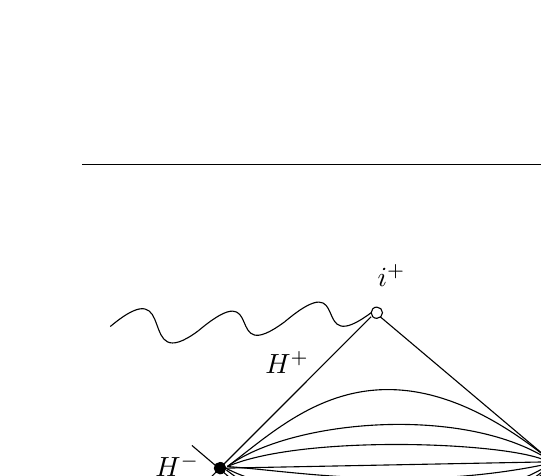
\begin{tikzpicture}[x=0.75pt,y=0.75pt,yscale=-1,xscale=1]
%uncomment if require: \path (0,369); %set diagram left start at 0, and has height of 369

%Straight Lines [id:da7009120242657934] 
\draw    (278.55,38.87) -- (361.32,108.73) ;
%Straight Lines [id:da1545469003174731] 
\draw    (274.17,38.87) -- (185.51,127.6) ;
%Straight Lines [id:da32591919942884995] 
\draw    (360.88,110.44) -- (286.87,181.67) ;
%Straight Lines [id:da17589607820200115] 
\draw    (187.82,100.86) -- (282.93,181.67) ;
%Shape: Ellipse [id:dp526980499146209] 
\draw   (274.17,36.92) .. controls (274.17,35.42) and (275.39,34.2) .. (276.91,34.2) .. controls (278.42,34.2) and (279.65,35.42) .. (279.65,36.92) .. controls (279.65,38.42) and (278.42,39.63) .. (276.91,39.63) .. controls (275.39,39.63) and (274.17,38.42) .. (274.17,36.92) -- cycle ;
%Shape: Ellipse [id:dp1657554694458303] 
\draw   (360.54,109.5) .. controls (360.54,108) and (361.77,106.78) .. (363.29,106.78) .. controls (364.8,106.78) and (366.03,108) .. (366.03,109.5) .. controls (366.03,111) and (364.8,112.21) .. (363.29,112.21) .. controls (361.77,112.21) and (360.54,111) .. (360.54,109.5) -- cycle ;
%Shape: Ellipse [id:dp2647324334508656] 
\draw   (282.59,182.86) .. controls (282.59,181.36) and (283.81,180.14) .. (285.33,180.14) .. controls (286.84,180.14) and (288.07,181.36) .. (288.07,182.86) .. controls (288.07,184.35) and (286.84,185.57) .. (285.33,185.57) .. controls (283.81,185.57) and (282.59,184.35) .. (282.59,182.86) -- cycle ;
%Shape: Ellipse [id:dp4671716682249334] 
\draw  [fill={rgb, 255:red, 0; green, 0; blue, 0 }  ,fill opacity=1 ] (198.63,111.79) .. controls (198.63,110.29) and (199.86,109.07) .. (201.37,109.07) .. controls (202.89,109.07) and (204.11,110.29) .. (204.11,111.79) .. controls (204.11,113.29) and (202.89,114.51) .. (201.37,114.51) .. controls (199.86,114.51) and (198.63,113.29) .. (198.63,111.79) -- cycle ;
%Curve Lines [id:da8859660872188637] 
\draw    (232.54,41.27) .. controls (266.47,12.77) and (243.33,59.84) .. (274.17,36.92) ;
%Curve Lines [id:da8496697188978106] 
\draw    (190.91,45.62) .. controls (224.84,17.12) and (201.7,64.19) .. (232.54,41.27) ;
%Curve Lines [id:da3523970653829964] 
\draw    (148.5,43.56) .. controls (182.43,15.06) and (160.07,68.54) .. (190.91,45.62) ;
%Curve Lines [id:da32631140641410417] 
\draw    (240.25,187.19) .. controls (274.18,158.69) and (251.04,205.76) .. (281.88,182.84) ;
%Curve Lines [id:da4087032012419831] 
\draw    (198.62,191.54) .. controls (232.55,163.04) and (209.41,210.11) .. (240.25,187.19) ;
%Curve Lines [id:da3758119768986756] 
\draw    (156.21,189.48) .. controls (190.14,160.98) and (167.78,214.46) .. (198.62,191.54) ;
%Curve Lines [id:da3939434625617442] 
\draw    (204.89,111.03) .. controls (235.73,88.11) and (320.43,81) .. (361.32,108.73) ;
%Curve Lines [id:da015977341407784174] 
\draw    (204.89,111.03) .. controls (235.73,88.11) and (279.23,41.69) .. (361.32,108.73) ;
%Curve Lines [id:da6668969025566764] 
\draw    (204.11,111.79) .. controls (240.25,130.66) and (329.7,132.42) .. (360.54,109.5) ;
%Curve Lines [id:da7638847895339227] 
\draw    (204.45,112.73) .. controls (281.11,170.38) and (330.04,133.36) .. (360.88,110.44) ;
%Curve Lines [id:da24654996057594847] 
\draw    (204.89,111.03) .. controls (242.56,94.75) and (348.59,99.57) .. (360.54,109.5) ;
%Curve Lines [id:da4948570185617598] 
\draw    (204.89,111.03) .. controls (235.62,113.08) and (294.22,123.78) .. (360.54,109.5) ;
%Straight Lines [id:da17198203973846304] 
\draw    (204.11,111.79) -- (361.32,108.73) ;


% Text Node
\draw (221.9,54.2) node [anchor=north west][inner sep=0.75pt]   [align=left] {$H^+$};
% Text Node
\draw (276.04,12.52) node [anchor=north west][inner sep=0.75pt]   [align=left] {$i^+$};
% Text Node
\draw (369.33,100.38) node [anchor=north west][inner sep=0.75pt]   [align=left] {$i^o$};
% Text Node
\draw (281.01,187.48) node [anchor=north west][inner sep=0.75pt]   [align=left] {$i^-$};
% Text Node
\draw (169,104) node [anchor=north west][inner sep=0.75pt]   [align=left] {$H^-$};


\end{tikzpicture}

\caption{Conformal diagram in Schwarzschild for simplicity. Every surface of constant $t$ gathers at spacelike infinity and at the "bifurcation sphere", the point at which the future horizon, $H^+$, and the past horizon, $H^-$, intersect.}
\end{figure}
If we work out $A$, we get 
\begin{align*}
    A &= \int (r_+^2 + a^2) sin\theta d\theta d\phi\\
    &= 4\pi(r_+^2 + a^2)\\
    &= 4\pi(M^2 + 2M \sqrt{M^2 - a^2}\: + M^2 - a^2 + a^2)\\
    &= 8\pi(M^2 + \sqrt{M^4 - J^2}\:)
\end{align*}
where $J = aM$.

By throwing an object into a black hole, we can change the mass and angular momentum of the black hole.
\[M \xrightarrow{} M + \delta M\]
\[J \xrightarrow{} J + \delta J\]
On HW7Q4, we find that $\delta M \geq \Omega_H \delta J$, where $\Omega_H = \omega\Bigr\rvert_{r\xrightarrow{}r_+} = \frac{a}{2Mr_+}$ is the horizon frequency.

What happens to $A$, the area of the black hole, when we add material? \begin{align*}
    \delta A &= 8\pi\delta(M^2+\sqrt{M^4-J^2}\:)\\
    &= 8\pi \frac{a}{\sqrt{M^2-a^2}}\frac{1}{\Omega_H}(\delta M-\Omega_H\delta J)
\end{align*}
Since $\delta M-\Omega_H\delta J > 0$ has to be greater than zero, even if $\delta M < 0$, $\delta A \geq 0$!

Let us define the \textbf{irreducible mass}, $M_{irr}$ as 
\begin{equation}
    M^2_{irr} = \frac{A}{16\pi} = \frac{1}{2}(M^2+\sqrt{M^4-J^2}\:) 
\end{equation}
which is a property of a black hole that can never decrease. We can see that 
\[M_{irr} \leq M\]
and when $J = 0$,
\[M_{irr} = M\]
This tells us that $M - M_{irr}$ is the rotational energy of the black hole. We can use $\delta M-\Omega_H\delta J$ and rearrange terms to see that 
\begin{equation}
    \frac{a}{2\sqrt{M^2-a^2}}\frac{4Mr_+}{a}=\frac{4Mr_+}{r_+-r_-}=\frac{1}{\kappa}
\end{equation}
where $\kappa$ is the surface gravity as defined before. From this, we can see that 
\begin{equation}
    \delta M = \frac{\kappa}{8\pi}(\delta A + \Omega_H\delta J)
\end{equation}
This is the first law of black hole thermodynamics.

A famous result by Stephen Hawking says that if the Weak Energy Condition (WEC) or the Strong Energy Condition (SEC) hold, then the black hole horizon always increases in area. This is as we saw above, that 
\[\delta A \geq 0\]
where $A$ is the sum of all areas of all individual black holes. This is the second law of black hole thermodynamics.

These laws of black hole thermodynamics are analagous to the first law of thermodynamics 
\begin{align*}
    \delta E &= T\delta S + \vec{\Omega}\cdot \vec{\delta J}\\
    &= T\delta S + P\delta V
\end{align*}
We can see that $\delta M$ is $\delta E$ of the spacetime, and $\delta A$ is related to $\delta S$. From this, we find an analogy that tells us that area is related to the entropy of the black hole and that the temperature is related to the surface gravity of the black hole. Specifically, 
\[A = \frac{S}{4}\]
\[T = \frac{\kappa}{2\pi}\]
in units where $k_B = 1$. But, attributing the temperature to the surface gravity is odd. What is going on here?

Using QFT and curved spacetime, Hawking showed that if you form a black hole from the collapse of a star, then at late times, you find that the black hole radiates due to quantum effects. A black hole is a blackbody with temperature $T = \frac{\kappa}{2\pi}$. Stellar black holes are at miniscule temperatures because $T \propto \frac{1}{M}$ since $\kappa \propto \frac{1}{M}$. In principle, if we could put a black hole in a region that was colder than itself, we would find that it radiates photons at a wavelength comparable to $\lambda \sim M$. This is called Hawking radiation.

\end{document}
